\section{Access management}\label{ms:sec:revoke}

Accessing a resource (or a macro-block in the resource, resp.) requires availability of all its fragments (its mini-blocks in all the fragments, resp.), and of the key used for encryption. Policy changes corresponding to granting access to new users can be simply enforced, as usual, by giving them the encryption key. In principle, policy changes corresponding to revocation of access would instead normally entail downloading the resource, re-encrypting it with a new key, re-uploading the resource, and distributing the new encryption key to all the users who still hold authorizations. Our approach enables the enforcement of access revocation to a resource by simply making any of its fragments unavailable to the users from whom the access is revoked. Since lack of a fragment implies lack of a mini-block for each macro-block of a resource, and lack of a mini-block prevents reconstruction of the whole macro-block, lack of a fragment equates to complete inability, for the revoked users, to reconstruct the plaintext resource or any portion of it. In other words, it equates to revocation.

\begin{figure}[!t]
\begin{footnotesize}
\hrule          %
\begin{tabbing}
\hfill\\
{\bf Encrypt}\\[1em]
\num{1:~}\= cut \resource\ in $\Mnum$ macro-blocks $\macroblock{0},\ldots,\macroblock{\Mnum-1}$\\[0.3em]
\num{2:~}\1 apply padding to the last macro-block \macroblock{\Mnum-1}\\[0.3em]
\num{3:~}\1 \var{IV} := randomly choose an initialization vector\\[0.3em]
\num{4:~}\1 \myfor\ $i=0,\ldots,\Mnum-1$ \com{do} \comm{encrypt macro-blocks}\\[0.3em]
\num{5:~}\2     \macroblock{\var{i}}$[[1]]$ := \macroblock{\var{i}}$[[1]]$ $\oplus$ \var{IV} \comm{{\sc xor} the first block with the IV}\\[0.3em]
\num{6:~}\2     {\bf Mix}(\macroblock{\var{i}}) \comm{encrypt the macro-block}\\[0.3em]
\num{7:~}\2     \var{IV} := \var{IV} $+$ 1 \comm{initialization vector for the next macro-block}\\[0.3em]
\num{8:~}\2     \myfor\ $j=0,\ldots,\mnumb^x-1$ \com{do} \comm{slicing}\\[0.3em]
\num{9:~}\3         \fragment{\var{j}}{}[\var{i}] := \macroblock{\var{i}}$[j]$
\end{tabbing}
\hrule
\vspace{.5em}
\end{footnotesize}
\caption{\label{ms:fig:algoenc}Algorithm for encrypting a resource \resource}
\end{figure}

\begin{figure*}[!t]
\setlength{\tabcolsep}{5pt}
\begin{tabular}{cc}
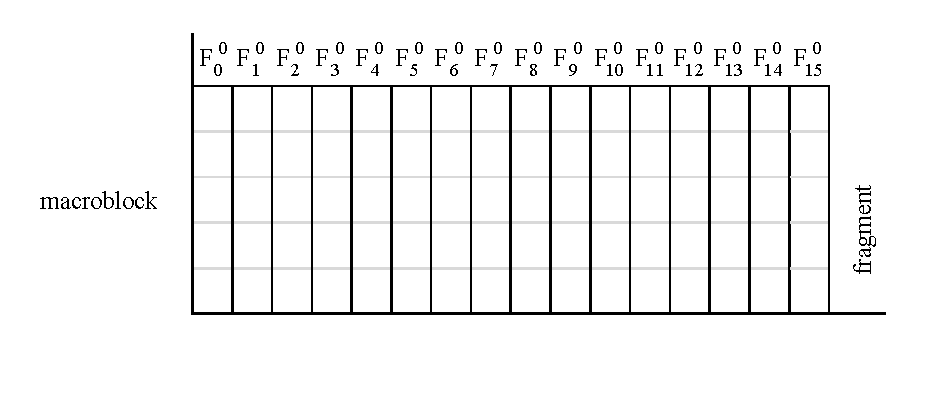
\includegraphics[width=0.48\columnwidth,valign=t]{figures/fig06a}&
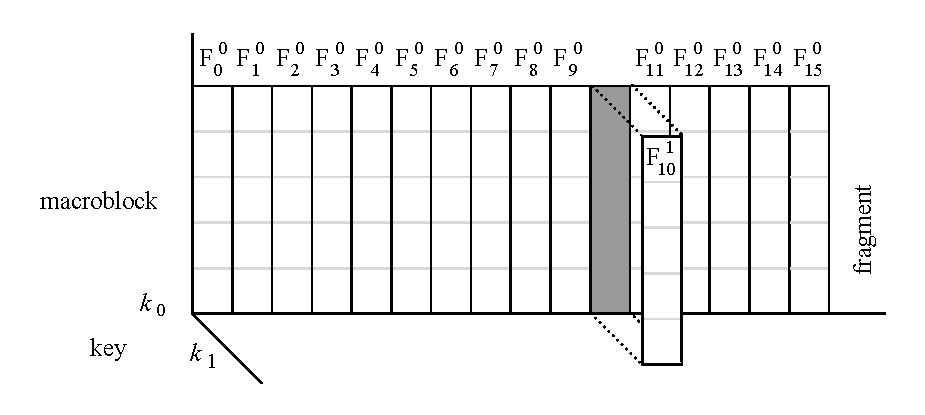
\includegraphics[width=0.48\columnwidth,valign=t]{figures/fig06b}\\
{\scriptsize (a)} & {\scriptsize (b)} \\
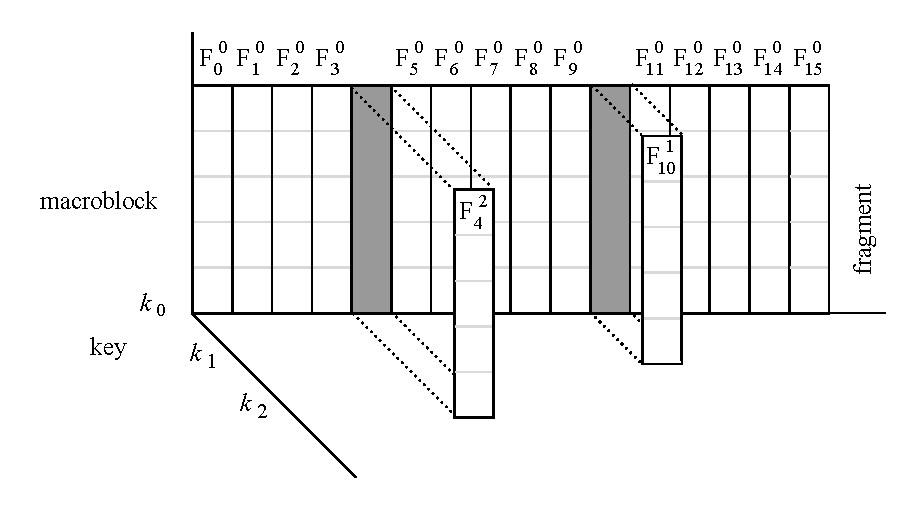
\includegraphics[width=0.48\columnwidth,valign=t]{figures/fig06c}&
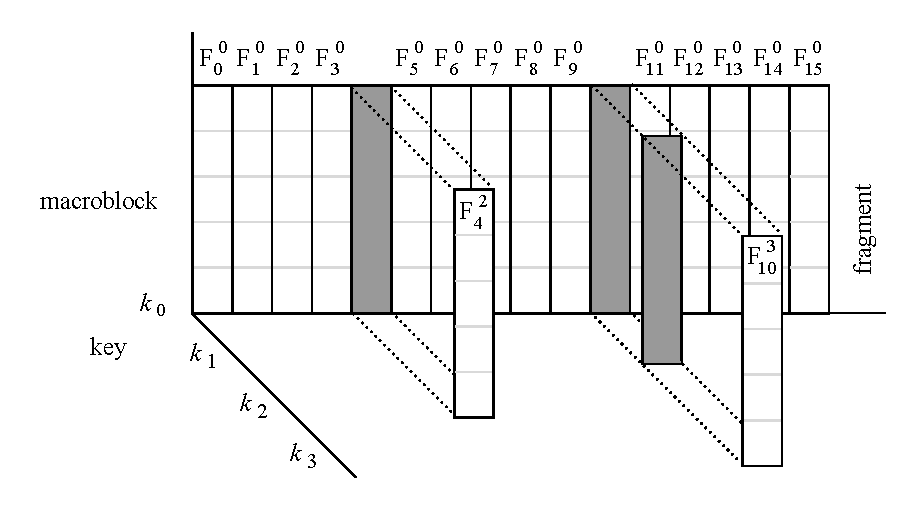
\includegraphics[width=0.48\columnwidth,valign=t]{figures/fig06d}\\
{\scriptsize (c)} & {\scriptsize (d)}\\
\end{tabular}
\caption{\label{ms:fig:pu}An example of fragments evolution}
\end{figure*}

Access revocations are then enforced by the data owner by randomly picking a fragment, which is then downloaded, re-encrypted with a new key (which will be made known only to users still authorized for the access), and re-uploaded at the server overwriting its previous version. While still requesting some download/re-upload, operating on a fragment clearly brings large advantages (in terms of throughput) with respect to operating on the whole resource (see Section~\ref{ms:sec:expe}). Revocation can be enforced on any randomly picked fragment (even if already re-written in a previous revocation) and a fresh new key is employed at every revoke operation. Figure~\ref{ms:fig:pu} illustrates an example of fragments evolution due to the enforcement of a sequence of revoke operations. Figure~\ref{ms:fig:pu}(a) is the starting situation with the original fragments computed as illustrated in Section~\ref{ms:sec:mixslice}. Figure~\ref{ms:fig:pu}(b-d) is the sequence of rewriting to enforce revocations, which involve, respectively, fragment \fragment{10}{}, re-encrypted with key \key{1}, fragment \fragment{4}{}, re-encrypted with key \key{2}, and fragment \fragment{10}{} again, now re-encrypted with key \key{3}. In the following, we use notation \fragment{\var{i}}{\var{j}} to denote a version of fragment \fragment{\var{i}}{} encrypted with key \key{j}, being \fragment{\var{i}}{0} the version of the fragment obtained through the mixing process. In the figure, the resource is represented in a three-dimensional space, with axes corresponding to fragments, macro-blocks, and keys. The re-writing of a fragment is represented by placing it in correspondence to the new key used for its encryption. The shadowing in correspondence to the previous versions of the fragments denote the fact that they are not available anymore as they are overwritten by the new versions.

Each revoke operation requires the use of a fresh new key and, due to policy changes, fragments of a resource might be encrypted with different keys. Such a situation does not cause any complication for key management, which can be conveniently and efficiently handled with a {\em key regression\/} technique~\cite{fkk06}. Key regression is an RSA-based cryptographically strong technique (the generated keys appear as pseudorandom) allowing a data owner to generate, starting from a seed \seed{0}, an unlimited sequence of symmetric keys $\key{0},\ldots,\key{u}$, so that simple knowledge of a key \key{i} (or the compact secret seed \seed{i} of constant size related to it) permits to efficiently derive all keys \key{j} with $j\leq i$. Only the data owner (who knows the private key used for generation) can perform forward derivation, that is, from \key{i}, derive keys following it in the sequence (i.e., \key{z} with $z\geq i$). Note instead that, not knowing the private key, users cannot perform forward derivation. The cost that users must pay for key derivation is small. On a single core, the computer we used for the experiments is able to process several hundred thousand key derivations per second.

With key regression, every user authorized to access a resource just needs to know the seed corresponding to the most recent key used for it (\seed{0} if the policy has not changed, \seed{3} in the example of Figure~\ref{ms:fig:pu}(d)). To this end, there is no need for key distribution, rather, such a seed can be stored in the resource descriptor and protected (encrypted) with a key corresponding to the resource's {\em acl\/} (i.e., known or derivable by all authorized users)~\cite{afb05,vldb07}. Enforcing revocation entails then, besides re-encrypting a randomly picked fragment with a fresh new key \key{i}, rewriting its corresponding seed \seed{i}, encrypted with a key associated with the new {\em acl\/} of the resource. Figure~\ref{ms:fig:revoke} illustrates the revocation process.

To access a resource, a user then first downloads the resource descriptor, to retrieve the most recent seed \seed{l}, and all the fragments. With the seed, she computes the keys necessary to decrypt fragments that have been overwritten, to retrieve their version encrypted with \key{0}. Then, she combines the mini-blocks in fragments to reconstruct the macro-blocks in the resource. She then applies mixing in decrypt mode to macro-blocks to retrieve the plaintext resource. Figure~\ref{ms:fig:access} illustrates the process to access a resource. 

Note that the size of macro-blocks influences the performance of both revoke and access operations. Larger macro-blocks naturally provide greater policy update performance as they decrease policy update cost linearly, with limited impact on the efficiency of decryption, since its cost increases logarithmically (Section~\ref{ms:sec:expe}).
